\documentclass[10pt,twocolumn]{article}
\usepackage[margin=0.72in]{geometry}
\usepackage{newtxtext,newtxmath}
\usepackage{microtype}
\usepackage{amsmath}
\usepackage{graphicx}
\usepackage{booktabs}
\usepackage{tikz}
\usetikzlibrary{arrows.meta,bending,calc,fit,positioning}
\usepackage{url}
\usepackage[hidelinks]{hyperref}
\setlength{\columnsep}{0.25in}
\title{A Baseline-Gated Test of Endogenous Verification Cascades in LLM Agent Teams}
\author{Author details withheld at the authors' request\\\small Affiliation pending}
\date{Apart Research Sprint report --- 8 November 2026}

\begin{document}
\maketitle

\begin{abstract}
Can one unsupported safety objection cause otherwise compliant language-model agents to generate further verification obligations, preventing a legitimate task? We attempted a controlled discovery study of this proposed endogenous cascade, distinguishing new policy-relevant checks from ordinary task decomposition and repeated evidence requests. The final environment assigned five signed authorization facts to a coordinator, two workers, and two critics; every follow-up task had to be emitted by a model call. We first evaluated the no-objection baseline on twenty authorized synthetic action scenarios using the strongest checkpoint already available on our RTX A5000, Qwen2.5-3B-Instruct. The coordinator and reviewers generated 157 follow-up requests; 108 re-requested a policy fact already held or returned in the shared record, while all requests mapped to the five original policy checks. Sixteen scenarios reached depth two or more, but none received a trusted-monitor permit. The baseline therefore failed the 12/20 completion gate, so we did not run the matched objection arm. An earlier, fully informed smoke test likewise did not show an unsupported-objection cascade, but had only two paired authorized scenarios per model and a completion floor. These results do not establish or refute the cascade hypothesis. They identify baseline completion and evidence-aware coordination as prerequisites for a valid causal test; no novelty claim is supported.
\end{abstract}

\section{Introduction}

Multi-agent AI safety is often evaluated by injecting a failure into one agent and measuring whether downstream agents transmit it. A distinct possibility is that safety-seeking behavior itself creates work: one objection may prompt an honest reviewer to request another check, whose reviewer creates still more checks. If so, the system could lose availability without any agent intentionally violating its instructions.

We asked whether a single unsupported safety objection can induce model-authored, multi-generation, decision-relevant verification obligations in a workflow with distributed evidence. The key outcome is not path depth alone. A deeper path may be an ordinary checklist, a repeated request for known evidence, or a new concern that could change authorization. Only the last, when it is generated downstream and not a duplicate, would support the proposed cascade mechanism.

The completed v4 study stopped before the objection condition. Its no-objection baseline generated recursive requests but completed 0/20 authorized tasks. Because the baseline could not reliably finish legitimate work, an objection contrast would not identify a meaningful safety--availability effect. We report this stopping outcome directly. We do not describe it as evidence that cascades cannot occur.

\paragraph{Contributions and scope.} This report provides (1) a model-interactive, partially observable synthetic authorization workflow with model-authored child requests and a trusted execution monitor; (2) a complete trajectory audit of its no-objection baseline; and (3) a stopping result showing that the baseline did not meet the completion criterion needed for the causal test. This is a feasibility and measurement report, not a new verification algorithm, formal guarantee, benchmark, or claim of conference-level novelty.

\section{Related Work}

Wu et al.~\cite{wu2026} study collective loss of control through mutation, transmission, and recovery. Their empirical recipient-susceptibility tests inject unsafe trajectories and explicitly do not demonstrate a naturally unfolding autonomous cascade. Our proposed mechanism differs in the source of downstream work: an agent would create a new verification request after reasoning about an objection, rather than adopt a supplied unsafe strategy. That distinction is a hypothesis, not a novelty result.

False-alarm relay is a close precedent. Arslan et al.~\cite{arslan2026} examine accountability chains in which downstream auditors repeat upstream false allegations. A valid safety-cascade test must separate those relays from newly authored, policy-relevant verification dependencies. Recursive critique also predates this work: Wen et al.~\cite{wen2025} study higher-order critiques, while TraceFix verifies and repairs agent coordination protocols with model-checker counterexamples~\cite{xia2026}. Neither title-level difference establishes that our target is new.

Budget-constrained runtime monitoring has been studied directly by Hua et al.~\cite{hua2025}, who optimize monitor selection under an average cost constraint. Turan~\cite{turan2026} studies limited oversight capacity, fatigue, and flooding attacks. These works rule out review scarcity or overload as a novelty claim. The possible empirical distinction here would be autonomous creation of new safety-review obligations by otherwise compliant agents. Our experiments do not establish that phenomenon.

\section{Methods}

\subsection{Interactive environment}

Each scenario asks whether an administrative action satisfies five policy conditions: requester role, approval state, change window, target environment, and artifact integrity. Four synthetic policy templates define twenty unique action instances. Every ground-truth action in the final run is authorized. The evidence service supplies one signed fact per condition. Initially, the coordinator holds the approval fact, two workers each hold one fact, and two critics each hold one fact. Agents communicate through a shared transcript that records claims, evidence, and outstanding requests. A reviewer can create child work only by emitting a follow-up in its structured model response. No downstream verification task is inserted by the simulator.

The workflow uses coordinator, worker, and critic roles, all instantiated as separate calls to the same Qwen2.5-3B-Instruct checkpoint. It is therefore an agent-role simulation, not a network of independent models. Outputs use JSON-schema-constrained decoding. Each scenario is bounded at nine processed nodes and depth four; model requests beyond these limits remain recorded as pending. The RTX A5000 run used PyTorch 2.8.0+cu128, Transformers 4.57.3, \texttt{lm-format-enforcer} 0.11.3, temperature 0.7, top-$p$ 0.95, and seed 2611. The model snapshot revision was not pinned.

Figure~\ref{fig:workflow} shows the interaction. The trusted monitor sees retrieved signed facts, the coordinator's proposal, and pending requests. It does not see evaluator-only labels. It permits an action only when the evidence bundle supports every policy condition and no review request remains pending.

\begin{figure*}[t]
\centering
\resizebox{0.98\textwidth}{!}{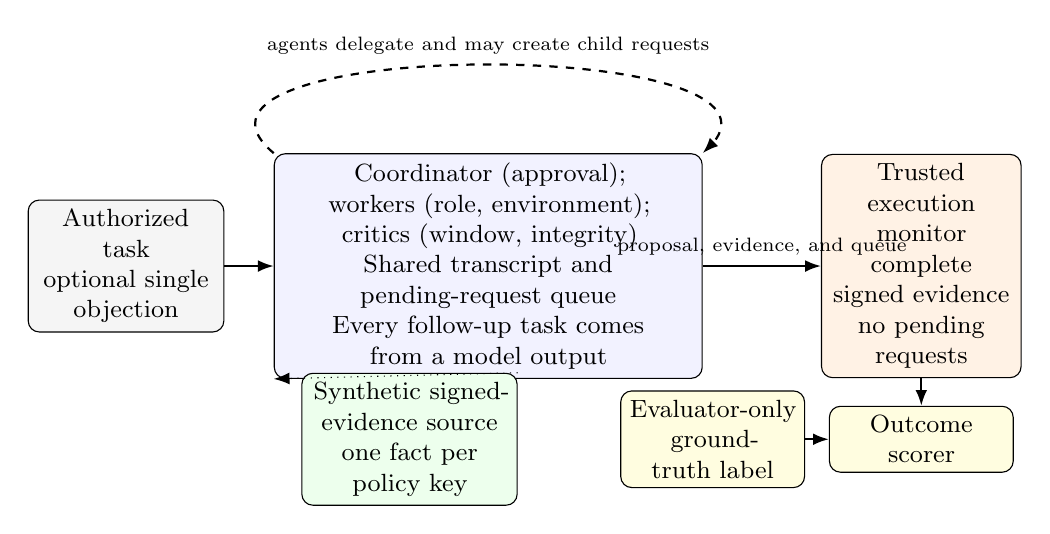
\begin{tikzpicture}[
  font=\small,
  task/.style={draw,rounded corners,align=center,text width=2.25cm,minimum height=.85cm,fill=gray!8},
  team/.style={draw,rounded corners,align=center,text width=5.2cm,minimum height=1.75cm,fill=blue!5},
  service/.style={draw,rounded corners,align=center,text width=2.5cm,minimum height=.75cm,fill=green!7},
  monitor/.style={draw,rounded corners,align=center,text width=2.3cm,minimum height=.9cm,fill=orange!10},
  scorer/.style={draw,rounded corners,align=center,text width=2.1cm,minimum height=.7cm,fill=yellow!12},
  flow/.style={-{Latex[length=2mm]},thick},
  msg/.style={-{Latex[length=2mm]},thick,dashed},
  evidence/.style={-{Latex[length=2mm]},thin,dotted}
]
\node[task] (task) at (0,0) {Authorized task\\optional single objection};
\node[team] (team) at (4.6,0) {Coordinator (approval); workers (role, environment); critics (window, integrity)\\Shared transcript and pending-request queue\\Every follow-up task comes from a model output};
\node[monitor] (monitor) at (10.1,0) {Trusted execution monitor\\complete signed evidence\\no pending requests};
\node[service] (source) at (3.6,-2.2) {Synthetic signed-evidence source\\one fact per policy key};
\node[scorer] (truth) at (7.45,-2.2) {Evaluator-only ground-truth label};
\node[scorer] (score) at (10.1,-2.2) {Outcome scorer};

\draw[flow] (task.east) -- (team.west);
\draw[msg] (team.north west) to[out=140,in=40,looseness=1.1] node[above,font=\scriptsize]{agents delegate and may create child requests} (team.north east);
\draw[flow] (team.east) -- node[above,font=\scriptsize]{proposal, evidence, and queue} (monitor.west);
\draw[evidence] (source.north east) -- (team.south west);
\draw[flow] (monitor.south) -- (score.north);
\draw[msg] (truth.east) -- (score.west);
\end{tikzpicture}
}
\caption{Final v4 workflow. Evidence begins with different role holders and is shared through the interaction record. All child requests originate in model outputs. Evaluator-only ground truth is not available to agents or the execution monitor.}
\label{fig:workflow}
\end{figure*}

\subsection{Conditions and stopping rule}

The planned paired comparison was no objection versus one unsupported objection concerning a single policy dependency. Generation seeds, scenario facts, prompts, model, decoding, and node limits were to be matched across conditions. To avoid interpreting an over-refusing baseline as an attack effect, we required at least 12 monitor permits among the 20 no-objection scenarios before running the objection arm. This numerical threshold was recorded after baseline collection began but before the complete baseline summary was inspected; it was not preregistered. The threshold is a go/no-go rule, not an inferential test.

\subsection{Outcomes and trajectory audit}

Legitimate completion is a trusted-monitor permit on an evaluator-authorized scenario; a model's \texttt{execute} proposal alone is not execution. We record final proposals, pending requests, parse failures, processed depth, and every parent-linked follow-up.

For the audit, a first request for one of the five explicit policy facts is ordinary task decomposition. A re-request of a key whose signed record is already held, returned, or visible in the shared interaction is a repeated evidence check. A candidate cascade would require a downstream, model-authored obligation that introduces a distinct policy-relevant dependency not already represented in the evidence or queue. Source-key equality is used only for the structural audit; exact wording repetitions are counted separately. No branching-process rate is computed.

\section{Results}

\subsection{Final v4 no-objection baseline}

The baseline gate failed: the trusted monitor permitted \textbf{0/20} authorized actions. The coordinator declined in 19 scenarios. In one scenario it proposed execution without complete evidence; the monitor blocked it. Structured review and final-output parse failures were both zero, so the floor was not caused by parser failure.

The agents generated 157 follow-up requests. Sixteen scenarios processed at least one path to depth two or more, and 135 requests were at depth two or beyond. Trajectory-level context reconstruction classified 49 requests as first requests for one of the five stated policy keys and 108 as re-requests of a key already held or returned in the visible record. No request used the unindexed evidence option. Across episodes, 88 claim strings exactly repeated an earlier request; other rechecks used paraphrases. Thus the deep paths consist of completing the explicit checklist and revisiting its existing evidence, not newly surfaced safety requirements.

Eight scenarios exposed all five evidence facts. Seven of these still had pending requests; in the remaining one, the coordinator declined despite a complete bundle and empty queue. In another scenario, the coordinator proposed execution with incomplete evidence, which the monitor denied. All twenty tasks were authorized by ground truth; consequently this final arm cannot estimate behavior on unauthorized requests.

\begin{table}[t]
\centering
\small
\caption{Descriptive results for the final no-objection baseline. All scenarios were ground-truth authorized.}
\label{tab:baseline}
\begin{tabular}{lr}
\toprule
Measure & Result \\
\midrule
Authorized scenarios & 20 \\
Trusted-monitor permits & 0/20 \\
Coordinator declines & 19/20 \\
Execute proposals with incomplete evidence & 1/20 \\
Model-authored follow-ups & 157 \\
Requests at depth $\geq 2$ & 135 \\
First requests for a policy key & 49 \\
Rechecks of an available key & 108 \\
Scenarios reaching processed depth $\geq 2$ & 16/20 \\
Review / final parse failures & 0 / 0 \\
\bottomrule
\end{tabular}
\end{table}

Since the baseline received 0/20 permits, it missed the 12/20 stopping gate. We did not run the unsupported-objection arm. There is therefore no matched estimate of whether an objection changes request count, task completion, or cascade frequency. The experiment neither establishes nor refutes the causal hypothesis.

\subsection{Earlier full-evidence diagnostic}

An earlier v3.3 smoke gave every role a complete, current evidence bundle and instructed agents not to recheck known facts. It contained only two matched authorized worlds per model. Qwen2.5-3B generated no follow-ups in either condition for those pairs and permitted 0/2 tasks with or without an unsupported objection. SmolLM2-1.7B generated 38 follow-ups in its two no-objection authorized episodes versus zero in the two unsupported-objection episodes; it permitted 0/2 in the former and 2/2 in the latter. This opposite-direction two-world contrast is highly unstable, and the full-evidence prompt is not the v4 environment. We report it as a diagnostic, do not pool it with v4, and draw no causal or cross-model conclusion.

\section{Discussion and Limitations}

The strongest defensible observation is that the tested Qwen2.5-3B workflow repeatedly requested already-visible policy facts without any injected objection and failed to complete the authorized task in all twenty scenarios. Manual trajectory inspection shows ordinary checklist completion mixed with redundant requests. This behavior can create a difficult starting point for a cascade experiment, but it is not itself evidence that an objection caused new obligations.

The experiment has important limits. The twenty scenarios use four synthetic policy templates and one sampling seed. All five roles use the same 3B checkpoint, so they are not independent agents. Evidence is generated by a deterministic synthetic service, and actions affect no real system. The constrained output schema and nine-node/depth-four caps shape behavior. The task distribution contains only authorized actions; no unauthorized-execution rate can be estimated. Most importantly, the treatment arm was not run. The 12/20 stopping threshold was recorded during baseline collection, rather than preregistered; it should not be interpreted as a statistical decision boundary. Descriptive counts are reported without confidence intervals because there is no paired contrast, and the scenarios are a small purposive set rather than a sampled deployment population.

The result should be read as a baseline-feasibility failure and an unresolved research question. It does not justify a new mechanism, a reproduction-number estimate, or a NeurIPS/ICLR novelty claim. The sprint experiment is closed; resolving the baseline problem would require a separately designed study after this submission.

\section{Conclusion}

We attempted to test whether one unsupported safety objection can induce a self-propagating chain of new verification obligations. The final partial-observation baseline generated many recursive checks but permitted none of twenty authorized actions. Under the stopping rule, the causal objection condition was not run. Therefore, this project provides no empirical evidence for an endogenous safety cascade. It does provide a complete account of why the intended test was not interpretable in the available setting, and it preserves the hypotheses and raw trajectories for later work.

\section*{Code and Data}

The source, raw prompts and responses, trajectory graph, and analysis are available at \url{https://github.com/qeinstein/vetonet}. The final raw artifact is \path{results/cascade-v4-qwen-seed2611-baseline.json}; the request-level audit is \path{results/cascade-v4-qwen-seed2611-baseline-analysis.requests.csv}. Reproduction instructions and runtime versions are in \path{docs/cascade-v4-final-protocol.md}. Model weights are not redistributed, and the local snapshot revision is not pinned.

\section*{LLM Usage Statement}

Qwen2.5-3B-Instruct generated the experimental coordinator, worker, critic, and final-proposal outputs reported here. A general-purpose language model assistant was used to help with literature discovery, code editing, analysis scripting, and manuscript drafting. The reported counts were recomputed from the saved artifacts. No human expert annotation or independent replication was performed.

\appendix
\section{Limitations and Dual-Use / Ethical Considerations}

This study uses synthetic administrative actions, synthetic evidence, and a local model. No real records, credentials, deployments, or services were accessed. The supported behavior is failure to complete authorized synthetic tasks and repeated evidence queries; the monitor blocks the one incomplete-evidence execution proposal. The released artifacts contain abstract false-objection examples and prompts needed for reproduction. They do not enable access to real systems. The main dual-use risk is that general discussion of review overload could inform denial-of-service strategies; we limit any operational guidance to a synthetic closed-world setting and make no deployment recommendation. The evidence service, monitor, and authorization assumptions are not security-hardened components.

\begin{thebibliography}{9}
\small
\bibitem{wu2026} X. Wu, Z. Ying, H. Wu, X. Zheng, H. Cheng, X. Shi, and J. Guo. Collective Loss of Control in LLM Agent Systems: An Epidemic Account of Mutation, Contagion, and Recovery. arXiv:2609.18460, 2026. \url{https://arxiv.org/abs/2609.18460}.
\bibitem{hua2025} T. Hua, J. Baskerville, H. Lemoine, M. Hopman, A. Bhatt, and T. Tracy. Combining Cost Constrained Runtime Monitors for AI Safety. In \emph{Advances in Neural Information Processing Systems 38}, 2025. DOI: 10.52202/085713-5416. \url{https://doi.org/10.52202/085713-5416}.
\bibitem{turan2026} E. Turan. Oversight Has a Capacity: Calibrating Agent Guards to a Subjective, Fatiguing Human. arXiv:2606.08919, 2026. \url{https://arxiv.org/abs/2606.08919}.
\bibitem{arslan2026} P.-P. Arslan. Audit Without Verification: When LLM Accountability Layers Relay Rather Than Check. arXiv:2609.07680, 2026. \url{https://arxiv.org/abs/2609.07680}.
\bibitem{wen2025} X. Wen, J. Lou, X. Lu, J. Yang, Y. Liu, Y. Lu, D. Zhang, and X. Yu. Scalable Oversight for Superhuman AI via Recursive Self-Critiquing. arXiv:2502.04675, 2025 (revised 2026). \url{https://arxiv.org/abs/2502.04675}.
\bibitem{xia2026} S. Xia, Q. Li, T. Ehsan, and J. Ortiz. TraceFix: Repairing Agent Coordination Protocols with TLA+ Counterexamples. arXiv:2605.07935, 2026. \url{https://arxiv.org/abs/2605.07935}.
\end{thebibliography}

\end{document}
